\chapter{Lineární programování}

Kapitola je zpracována z \cite{semidefinite-optimization-and-convex-algebraic-geometry}, \cite{understanding-and-using-linear-programming} a \cite{ko}.

\section{Primární úloha}

Úlohou lineárního programování rozumíme minimalizaci nebo maximalizaci lineární \textbf{účelové funkce} vzhledem k afinním \textbf{omezením}, kde tato omezení jsou dána soustavou lineární rovnic a nerovnic. Úlohu lineárního programování lze formulovat v několika ekvivalentních tvarech, které se liší zadáním omezení. Úloha v \textbf{kanonickém tvaru} má svá omezení dána soustavou lineárních nerovnic $Ax \leq b$. Tedy
\begin{equation}\tag{LP-P}
    \max \left\{ c^T x \mid Ax \leq b, x \geq 0 \right\},
    \label{eq:LP-P}
\end{equation}
kde $A \in \mathbb{R}^{m \times n}$, $b \in \mathbb{R}^n$, $x \in \mathbb{R}^n$ a $c \in \mathbb{R}^n$. \textbf{Přípustná množina řešení} je průnikem poloprostorů, které jsou definovány soustavou nerovnic $Ax \leq b$ a \textbf{nezáporného ortantu}, tj. množiny $\left\{ x \in \mathbb{R}^n \mid x_i \geq 0, i = 1, \dots, n \right\}$. Obě tyto množiny jsou konvexní a tedy i jejich průnik je rovněž konvexní množina. Dále, protože přípustnou množinu máme popsanou soustavou konečně mnoha lineárních nerovnic, geometricky se na úlohu \ref{eq:LP-P} díváme jako na maximalizaci lineární funkce přes polyedr, který je definován touto soustavou.

\begin{pr}
Mějme následující maximalizační úlohu.
\begin{equation}\tag{P1}
    \begin{split}
        \max x_1 + x_2 &       \\
        - x_1 + 3 x_2  &\leq 4 \\
        4 x_1 -   x_2  &\leq 6 \\
        x &\geq 0.
    \end{split}
    \label{eq:P1}
\end{equation}

Přípustná množina řešení je zobrazena na obrázku~\ref{fig:ex1}. Řešením úlohy je vektor $x^* = (2, 2)$ s cenou $4$.
\end{pr}

\begin{figure}[h!]
    \centering
    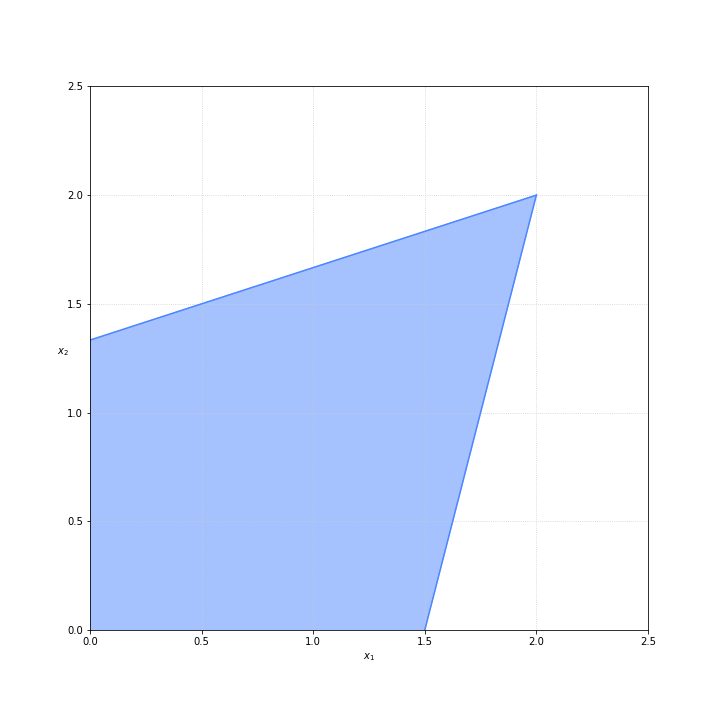
\includegraphics[width=0.5\textwidth]{img/ex1.png}   
    \caption{Přípustná množina řešení k úloze~\ref{eq:P1}.}
    \label{fig:ex1}
\end{figure}

\section{Dualita}

Pomocí Lagrangeovy duality odvodíme duální úlohu k primární úloze~\ref{eq:LP-P}. Máme tedy optimalizační úlohu
\begin{equation*}
    \min \left\{ -c^Tx \mid Ax \leq b, x \geq 0 \right\}.
\end{equation*}

\noindent Pro ní vytvoříme Lagrangeovu funkci
\begin{equation*}
    \begin{split}
        L(x, \lambda) &= -c^Tx + \lambda^T \left( Ax - b \right) - \lambda^Tx \\
                      &= -b^T\lambda + \left( A^T\lambda - c - \lambda \right)^Tx.
    \end{split}
\end{equation*}

\noindent Z Lagrangeovy funkce přejdeme k duální funkci
\begin{equation*}
    \begin{split}
        d(\lambda)  &= \inf_x L(x, \lambda) \\
                    &= \inf_x -b^T\lambda + \left( A^T\lambda - c - \lambda \right)^Tx \\
                    &=
                    \begin{cases}
                        -b^T\lambda & \text{pokud } A^T\lambda - c - \lambda = 0, \\
                        -\infty     & \text{jinak}.
                    \end{cases}
    \end{split}
\end{equation*}

\noindent Tu nakonec použijeme v duální úloze
\begin{equation*}
    \max \left\{ -b^T\lambda \mid A^T\lambda -c - \lambda = 0 \right\}
\end{equation*}

\begin{equation*}
    \max \left\{ -b^T\lambda \mid A^T\lambda \geq c, \lambda \geq 0 \right\}
\end{equation*}

\begin{equation}\tag{LP-D}
    \min \left\{ b^T\lambda \mid A^T\lambda \geq c, \lambda \geq 0 \right\}
    \label{eq:LP-D}
\end{equation}

\noindent Dostáváme tedy duální úlohu~\ref{eq:LP-D} k primární úloze~\ref{eq:LP-P}.

\begin{pr}
Duální úloha k \ref{eq:P1} je v následujícím tvaru.
\begin{equation}\tag{P2}
    \begin{split}
        \min 4 y_1 + 6 y_2 &       \\
        - y_1 + 4 y_2      &\geq 1 \\
        3 y_1 -   y_2      &\geq 1 \\
        y &\geq 0.
    \end{split}
    \label{eq:P2}
\end{equation}

Přípustná množina řešení je zobrazena na obrázku~\ref{fig:ex2}. Řešením úlohy je vektor $y^* \approx (0.4546, 0.3636)$ s cenou $4$.
\end{pr}

\begin{figure}[h!]
    \centering
    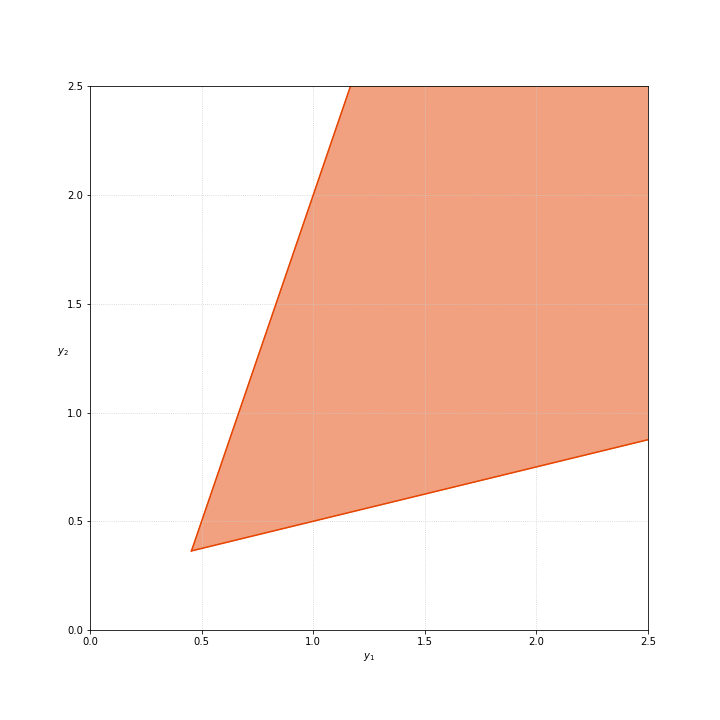
\includegraphics[width=0.5\textwidth]{img/ex2.png}   
    \caption{Přípustná množina řešení k úloze~\ref{eq:P2}.}
    \label{fig:ex2}
\end{figure}

Všimněme si, že v příkladech \ref{eq:P1} a \ref{eq:P2} mají řešení $x^*$ i $y^*$ stejnou cenu. To není náhoda a tento fakt je obsahem silné věty o dualitě lineárního programování, kterou dokázal v roce 1947 John von Neumann. Začneme slabou větou o dualitě lineárního programování.

\begin{vt2}[Slabá věta o dualitě.]
    Nechť $\tilde{x}$ je přípustné řešení \ref{eq:LP-P} a $\tilde{y}$ je přípustné řešení \ref{eq:LP-D}. Potom $c^T \tilde{x} \leq b^T \tilde{y}$.
\end{vt2}

Tedy každé přípustné řešení $\tilde{y}$ duální úlohy \ref{eq:LP-D} nám dává horní odhad na maximum účelové funkce primární úlohy \ref{eq:LP-P}. Graficky můžeme slabou větu o dualitě interpretovat jako na obrázku~\ref{fig:weak_duality}. Zatím tedy nevíme, zda vždy existují přípustná (optimální) řešení $x^*$ pro úlohu \ref{eq:LP-P} a $y^*$ pro úlohu \ref{eq:LP-D}, pro která platí $c^T x^* = b^T y^*$. Kladnou odpověď dostaneme z již zmíněné silné věty od dualitě.

\begin{figure}[h!]
    \centering
    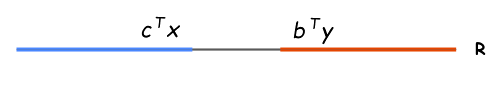
\includegraphics[width=0.5\textwidth]{img/weak_duality.png}   
    \caption{Slabá věta o dualitě.}
    \label{fig:weak_duality}
\end{figure}

\begin{vt2}[Silná věta o dualitě.]
    Jestliže úlohy \ref{eq:LP-P} a \ref{eq:LP-D} mají přípustná řešení. Potom
    $$
        \max \left\{ c^T x \mid Ax \leq b, x \geq 0 \right\} = \min \left\{ b^T y \mid A^T y \geq c, y \geq 0 \right\}.
    $$ 
\end{vt2}
Se znalostí silné věty o dualitě můžeme obrázek~\ref{fig:weak_duality} upravit na obrázek~\ref{fig:strong_duality}.

\begin{figure}[h!]
    \centering
    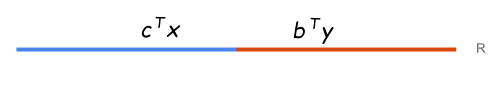
\includegraphics[width=0.5\textwidth]{img/strong_duality.png}
    \caption{Ceny přípustných řešení primární a příslušné duální úlohy.}
    \label{fig:strong_duality}
\end{figure}

\section{Komplementární skluzovost}

Pro odvození tzv. podmínky komplementární skluzovosti nejprve převedeme úlohy \ref{eq:LP-P} a \ref{eq:LP-D} do jiných tvarů. V primární úloze povolíme $x \in \mathbb{R}^n$. Tedy primární úloha je ve tvaru

\begin{equation}\tag{LP-P2}
    \max \left\{ c^T x \mid Ax \leq b \right\}.
    \label{eq:LP-P2}
\end{equation}
A příslušná duální úloha je ve tvaru

\begin{equation}\tag{LP-D2}
    \min \left\{ b^T y \mid A^T y = c, y \geq 0 \right\}.
    \label{eq:LP-D2}
\end{equation}

Nechť $\tilde{x}$ je připustné řešení a $x^*$ je optimální řešení úlohy \ref{eq:LP-P2}, $\tilde{y}$ je přípustné řešení a $y^*$ je optimální řešení úlohy \ref{eq:LP-D2}. \textbf{Dualitní rozdíl} $\tilde{x}$ a $\tilde{y}$ je číslo $b^T \tilde{y} - c^T \tilde{x} \geq 0$. Ze silné věty o dualitě samozřejmě plyne, že pro optimální řešení $x^*$ a $y^*$ je dualitní rozdíl roven $0$. Vyjdeme z dualitního rozdílu optimálních řešení.
$$
    b^T y^* - c^T x^* = y^{*^T} b - y^{*^T} A x^* = y^{*^T} \left( b - A x^* \right) = 0.
$$
Poslední rovnost přepíšeme maticově
$$
    \left[ y_1^*, \dots, y_m^* \right] \left(
        \begin{bmatrix}
            b_1    \\
            \vdots \\
            b_m
        \end{bmatrix}
        -
        \begin{bmatrix}
            a_{11} & \dots & a_{1n} \\
            \vdots & \     & \vdots \\
            a_{m1} & \dots & a_{mn}
        \end{bmatrix}
        \begin{bmatrix}
            x_1^*  \\
            \vdots \\
            x_n^*
        \end{bmatrix}
    \right)
    =
    \begin{bmatrix}
    0      \\
    \vdots \\
    0
    \end{bmatrix}.
$$
Dostáváme tedy soustavu rovnic $y_i^* \left( b_i - a_{i\_} x^* \right) = 0$, kde $i = 1, \dots, m$. Tedy buď $y_i^* = 0$ nebo $ b_i - a_{i\bullet} x^* = 0$ ($a_{i\bullet}$ značí $i$-tý řádek matice $A$). \textbf{Podmínka komplementární skluzovosti} je splněna, jestliže pro přípustná řešení $\tilde{x}, \tilde{y}$ platí buď $\tilde{y}_i = 0$ nebo $b_i - a_{i\bullet} \tilde{x} = 0$, $i = 1, \dots, m$. Pokud nastane $b_i - a_{i\bullet} \tilde{x} = 0$, potom říkáme, že \textbf{vazba $a_{i\_} \tilde{x} \leq b_i$ je aktivní}.

\begin{vt2}
    Nechť $\tilde{x}$ je přípustné řešení \ref{eq:LP-P2} a $\tilde{y}$ je přípustné řešení \ref{eq:LP-D2}. Potom $\tilde{x}, \tilde{y}$ jsou optimální právě tehdy, když platí podmínka komplementární skluzovosti.
\end{vt2}
